\documentclass{article}
\usepackage[UTF8]{ctex}
\usepackage{booktabs}
\usepackage{multirow}
\usepackage[table,xcdraw]{xcolor}
\usepackage{fancyhdr}
\usepackage{amsmath}
\usepackage[linesnumbered,lined,ruled,vlined,commentsnumbered]{algorithm2e}
\usepackage{tabu}
\usepackage{listings}
\usepackage{float}
\usepackage{graphicx}
\usepackage{pstricks}
\usepackage{pst-node}
\usepackage{courier}
\usepackage{fontspec}
\usepackage{lipsum}
\usepackage{enumerate}
\usepackage{cite}
\usepackage[section]{placeins}
\usepackage[hyphens]{url}
\usepackage[UKenglish]{babel}% http://ctan.org/pkg/babel
\usepackage[UKenglish]{isodate}% http://ctan.org/pkg/isodat

\usepackage{color}
\lstset{
  language=C++,                % choose the language of the code
  numbers=left,                   % where to put the line-numbers
  stepnumber=1,                   % the step between two line-numbers.        
  numbersep=5pt,                  % how far the line-numbers are from the code
    % choose the background color. You must add \usepackage{color}
  showspaces=false,               % show spaces adding particular underscores
  showstringspaces=false,         % underline spaces within strings
  showtabs=false,                 % show tabs within strings adding particular underscores
  tabsize=2,                      % sets default tabsize to 2 spaces
  captionpos=b,                   % sets the caption-position to bottom
  breaklines=true,                % sets automatic line breaking
  breakatwhitespace=true,         % sets if automatic breaks should only happen at whitespace
  title=\lstname,                 % show the filename of files included with \lstinputlisting;
    basicstyle=\ttfamily,
    keywordstyle=\color{blue}\ttfamily,
    stringstyle=\color{red}\ttfamily,
    %commentstyle=\color{green}\ttfamily,
    commentstyle=\color[RGB]{0,146,146},
    morecomment=[l][\color{magenta}]{\#}
}  

\newrgbcolor{myblue}{0.7 0.8 1}
\def\NODE(#1,#2)#3{\cnode(#1,#2){.35cm}{#3}\rput(#1,#2){#3}}
\def\MARKED(#1,#2)#3{\cnode[fillstyle=solid,fillcolor=myblue](#1,#2){.35cm}{#3}\rput(#1,#2){#3}}
\def\ya{3.6}\def\yb{2.4}\def\yc{1.2}\def\yd{0}\def\yy{4.6}

% Default fixed font does not support bold face
\DeclareFixedFont{\ttb}{T1}{txtt}{bx}{n}{12} % for bold
\DeclareFixedFont{\ttm}{T1}{txtt}{m}{n}{12}  % for normal

% Custom colors
\definecolor{deepblue}{rgb}{0,0,0.5}
\definecolor{deepred}{rgb}{0.6,0,0}
\definecolor{deepgreen}{rgb}{0,0.5,0}

% Python style for highlighting
\newcommand\pythonstyle{\lstset{
        language=Python,
        basicstyle=\ttm,
        otherkeywords={self},             % Add keywords here
        keywordstyle=\ttb\color{deepblue},
        emph={MyClass,__init__},          % Custom highlighting
        emphstyle=\ttb\color{deepred},    % Custom highlighting style
        stringstyle=\color{deepgreen},
        frame=tb,                         % Any extra options here
        showstringspaces=false            % 
}}

% Python environment
\lstnewenvironment{python}[1][]
{
    \pythonstyle
    \lstset{#1}
}
{}

% Python for external files
\newcommand\pythonexternal[2][]{{
        \pythonstyle
        \lstinputlisting[#1]{#2}}}

% Python for inline
\newcommand\pythoninline[1]{{\pythonstyle\lstinline!#1!}}
\begin{document}
\SetKwProg{Fn}{Function}{}{} 
\SetKwFunction{lis}{LIS}
\setsansfont{Verdana}
\setmonofont{Courier}
\SetAlFnt{\ttfamily}
\SetKwSty{texttt}
%\SetFuncArgSty{texttt}
\SetArgSty{texttt}

\setkeys{Gin}{keepaspectratio, width=1 \textwidth}

\renewcommand{\figurename}{\textbf{Diagram}}

\fancyhf{}
\rhead{OOP}
\lhead{STL Allocator With Memory Pool}
\cfoot{\thepage}

\renewcommand\contentsname{Content}
\renewcommand{\lstlistingname}{\textbf{Code}}

\title{\textbf{STL Allocator with Memory Pool} \\
	\large Object Oriented Programming\\
	\large Final Project}
\date{\today}

\maketitle
\thispagestyle{empty}
\newpage
\pagestyle{plain}

\tableofcontents
\thispagestyle{empty}
\newpage
\setcounter{page}{1}
\pagestyle{fancy}

\section{Introduction}
\subsection{Background}
Up to now, as for allocating memory space, I believe, most of us just simply use \texttt{new/malloc} or \texttt{delete/free} So far, since only small program are built, so good. The only thing we need to do is to make a system call. Even when some careless programmer forgets to verify whether space is allocated normally, it always works. 

However, hidden trouble exists. 
\begin{itemize}
	\item First, take implement of those system calls into consideration. 
	
	Take \texttt{malloc/free} as an example. There is a free linked list which links free memory blocks. When \texttt{malloc} function is called, system will use some optiminum algorithm to search for a suitable space. If necessary, it will split a space block, return one to caller, and add another to linked list. When \texttt{free} function is called, system will links the space which needs to be deallocated to free lists. 
	
	Thus, when it comes to a special program, where frequent \texttt{malloc/free} calls for small object occur, the free list will finally hold numberous fragments. Then when another \texttt{malloc} call occurs, system must arrange those fragments first, the completment of space allocation will be delayed. 
	
	\item Second, it's fact that even with no rearrangment, call for those function takes lots of time. When numberous calls occur, extra time are consumed.
\end{itemize}

According to the hidden trouble above, obviously, if a program needs to make numberous allocataion and deallocation calls, default space allocation methods are not recommendable. We must construct new memory management.
\subsection{Memory Pool}
Memory pool, also called fixed-size blocks allocation, is a good option [1]. In order not to suffer from fragmentation and to speed up memory allocation, it preallocates a number of memory blocks with some fixed size. 

Then application can allocate, access and free memory through the following interface:

\begin{enumerate}
	\item \textbf{Allocate memory from the pools. }
	
	The function will determine the pool where the required block fits in. If all blocks of that pool are already reserved, the function tries to find one in the next bigger pool(s).
	\item \textbf{Get an access pointer to the allocated memory.}
	\item \textbf{Free the formerly allocated memory block by return it to pool.}
\end{enumerate}

In general, pool allocators can help with allocating/freeing allocations of a certain size, in any order, in O(1) time.

\subsection{Our Goal}
Our task is to implement an allocator with memory pool to support \texttt{std::vector} and \texttt{std::list}.

The requirement is listed below:
\begin{itemize}
	\item \textbf{The allocator should optimize memory allocation speed usind memory pool.}
	\item \textbf{The allocator should support arbitrary memory size allocation request.}
\end{itemize}

Then we should test the ability of the allocator with 10000 times of various size of vector construction and destruction.

\section{Our Allocator with Memory Pool}

\subsection{STL Allocator Interface Implement}

In C++ computer programming, \texttt{allocator}s are an important component of the C++ Standard Library. STL provides several data strucures referred to as containers. And a common trait among these containers is their ability to change size during the execution of the program. To achieve this, some form of dynamic memory allocation is usually required. Allocators handle all the requests for allocation and deallocation of memory.

Any class that fulfills the \textbf{allocator requirements} can be used as an allocator. In particular, a class \texttt{A} capable of allocating memory for an object of type \texttt{T}  must provide types for generically declaring objects and references (or pointers) to objects of type \texttt{T}, type that represent the largest size for an object in the allocation modele defined by \texttt{A}, and type that can represent the difference between any two pointers in the allocation model.
	\begin{lstlisting}
	A::pointer
	A::const_pointer
	A::reference
	A::const_reference
	A::value_type
	A::size_type
	A::difference_type
	\end{lstlisting}
STL separates the process of \texttt{new} or \texttt{delete} an object into two steps. As for \texttt{new} an object, first we allocate suitable space by \texttt{allocate} function, then we call \texttt{construct} function to construct object. And the \texttt{delete} function is similar. Thus we are able to optimize the first step seperately.

These two functions are to construct or destroy an object.  
\begin{lstlisting}
template <typename T> void A::construct(A::pointer p, A::const_reference t) { new ((void*) p) T(t); } 
template <typename T>
void A::destroy(A::pointer p){ ((T*)p)->~T(); } 
\end{lstlisting}
These two functions are to perform allocation and deallocation. The way we allocate memory is realized by these two functions. 

\begin{lstlisting}
void A::deallocate(A::pointer Ptr, A::size_type Count)
A::pointer A::allocate(A::size_type Count)
\end{lstlisting}

In our ideal, the two functions should work with memory pool. However, in one of the STL versions, P.J. Plauger version, which is adopted by Visual Studio, these two functions simply package \texttt{new / delete}, and make no effort to optimize memory allocation. Later, we will design the two functions and memory pool with inspiration of SGI STL, and optimize memory allocation.

Inspired by \texttt{alloc} in SGI STL [2], we design our own allocator. The three major member functions are listed below. The class memory pool will be stated in next sub-section.

\begin{lstlisting}
void deallocate(pointer Ptr, size_type Count) {
	size_type Size = Count * sizeof(T);
	memoryPool::deallocate(Ptr, Size);
}
\end{lstlisting}
\begin{lstlisting}
_DECLSPEC_ALLOCATOR pointer allocate(size_type Count) {
	void *Ptr = NULL;
	size_type Size = Count * sizeof(T);
	if (Count) {
		Ptr = memoryPool::allocate(Size);
	}
	return static_cast<pointer>(Ptr);
}
\end{lstlisting}
\begin{lstlisting}
_DECLSPEC_ALLOCATOR pointer allocate(size_type Count, const void*) {
	return allocate(Count);
}
\end{lstlisting}
These are some extra member functions that class \texttt{A} needs.

This function is to get the largest number of objects of type T that could be expected to be successfully allocated.
\begin{lstlisting}
A::max_size(){ return UINT_MAX / sizeof(T); }
\end{lstlisting}
This function is to denote the address of an object.
\begin{lstlisting}
A::pointer A::address(A::reference V){return &V} 
\end{lstlisting}
In order to enable the possibility of obtaining a related allocator, Allocators are also required to supply a template member:
\begin{lstlisting}
template <typename U> struct A::rebind { typedef A<U> other; };
\end{lstlisting}
\subsection{Our Memory Pool}
The declaration of class \texttt{memoryPool}:
\begin{lstlisting}
class memoryPool {
	typedef size_t size_type;
	
public:
	static void *allocate(size_type N);
	static void deallocate(void *Ptr, size_type N);
	
private:
	enum{Align = 8};
	enum{MaxBytes = 4096};
	enum{SecondMaxBytes = 40960};
	enum{NFreeLists = MaxBytes / Align};
	enum{BigFreeLists = (SecondMaxBytes - MaxBytes)/Align};
	enum{NumOfObj = 20};
	enum{Increment = 8};
	
	#define roundUp(x)	 (((x) + Align - 1) & (~(Align - 1)))
	
	union Obj {
	Obj * freeListLink;
	char Data;
	};
	
	static char *startFree;
	static char *endFree;
	static Obj * freeList[NFreeLists];
	static Obj * BFreeList[BigFreeLists];
	static int freeListCnt[NFreeLists];
	static size_type heapSize;
	
	static inline size_type freeListIndex(size_type N);
	static void *refill(size_type N);
};
\end{lstlisting}

Here, the two public member functions \texttt{void *allocate(size\_type N)} and \texttt{void deallocate(void *Ptr, size\_type N)} are called in our allocator as is stated earlier.

In class memory pool, \texttt{allocate} and \texttt{deallocate} functions are both realized by three allocation methods in order to avoid memory fragments, speed up allocation, and reduce extra needed space. When the required space is big enough, we adopt the first allocation strategy: simply use \texttt{new} function to get space. If the required space is bigger than fisrt threshold we set, but smaller than second threshold, we adopt the second strategy with memory pool. If the required space is bigger than second threshold, which means it is big enough, we will adopt final strategy with memory pool too, as \ref{framework} shows. 

\begin{figure}
	\centering
	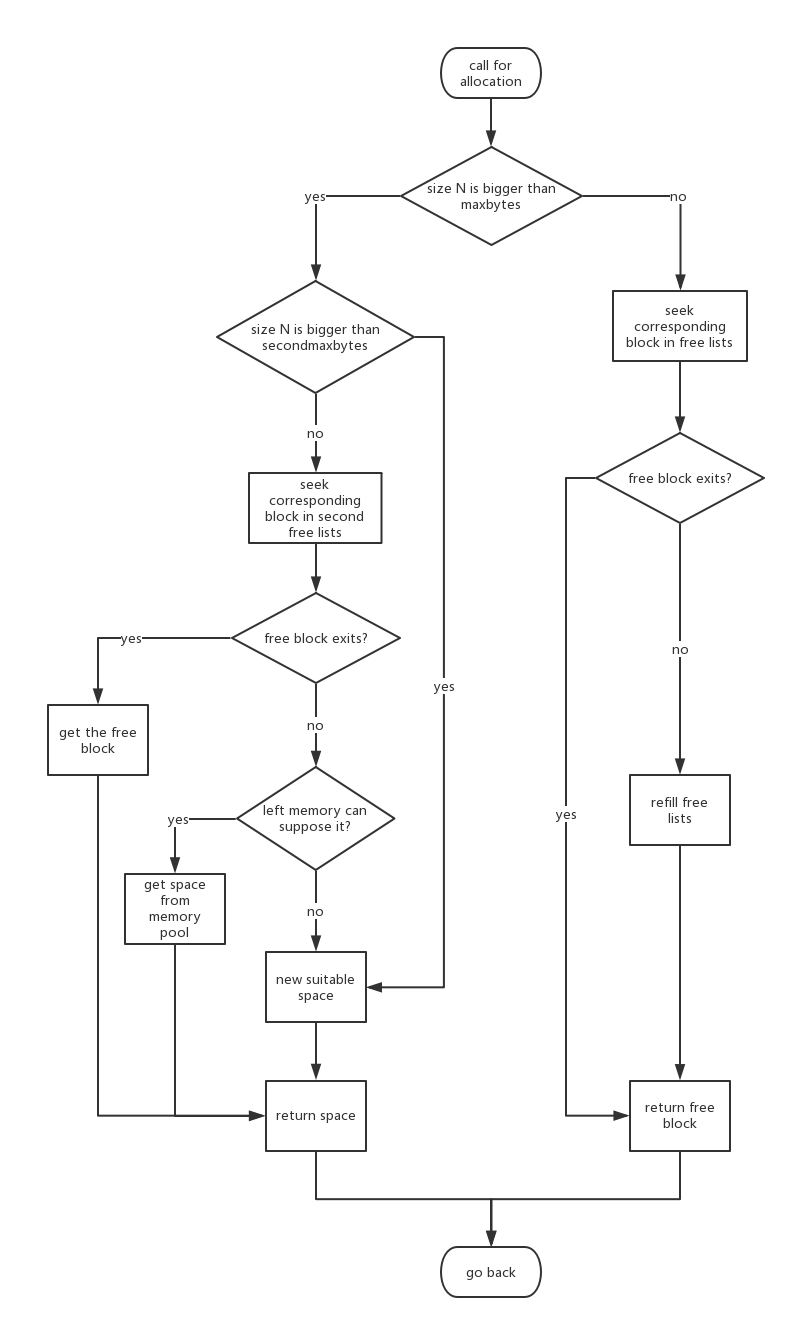
\includegraphics[]{frame.png}
	\caption{Allocator framework\label{framework}}
\end{figure}

\subsubsection{First-level allocation}
In first-level allocation, since time of allcation for big space is much less than that for small space, we set a parameter \texttt{MaxBytes} as threshold, and if allocation block is bigger than the threshold, we just use \texttt{new} to allocate. 

We design this method because as for big space block, compared with much more extra space to manage memory pool, the time consumed with directly allocation is acceptable, let alone that the requirment time is less.

Here \texttt{N} is the required bytes.
\begin{lstlisting}
(void *)::operator new(N);
\end{lstlisting}

Here \texttt{Ptr} is a pointer pointing to the space needing free.
\begin{lstlisting}
::operator delete(Ptr);
\end{lstlisting}
\subsubsection{Second-level allocation}
In second-level allocation, since in test program, most of space required is for rather small object, and the times of the new operation and delete operation of small objects are so frequent, numberous space that could be saved for later use is wrongly freed. Thus, lots of time is wasted. So in this level, we design a allocation method to keep a free list to hold small space blocks and maintain a memory pool:

Everytime when a small block is required, allocate a big block, and maintain corresponding free list. Next time when same block is required, return one block held in free list. If it needs to be freed, allocator will put it back to free list, waiting for next call. And for sake of more convienent management, we will align space capacity by 8 bytes. For example, if client requires space with 30 bytes, we will regard it as 32 bytes.  If the parameter is 4 bytes, then too many linked lists should be managed. If it is 16 bytes, then wasted space is too big. Thus we choose 8 bytes to align. In this way, considering that \texttt{int, float} and pointer all occupy 4 bytes, the waste is acceptable, and management cost is also appropriate.


\begin{itemize}
	\item{Freelists}
	
	\texttt{FreeLists} is a pointer array. It's element type is pointer implemented by union  pointing to a linked list as \ref{freelist} shows. Each linked list holds free small blocks with a corresponding fixed size like \ref{linkedlist} shows. And we use \texttt{union} to implement pointer, in order to reduce extra cost for maintainment of freelists. 
	\begin{figure}
		\centering
		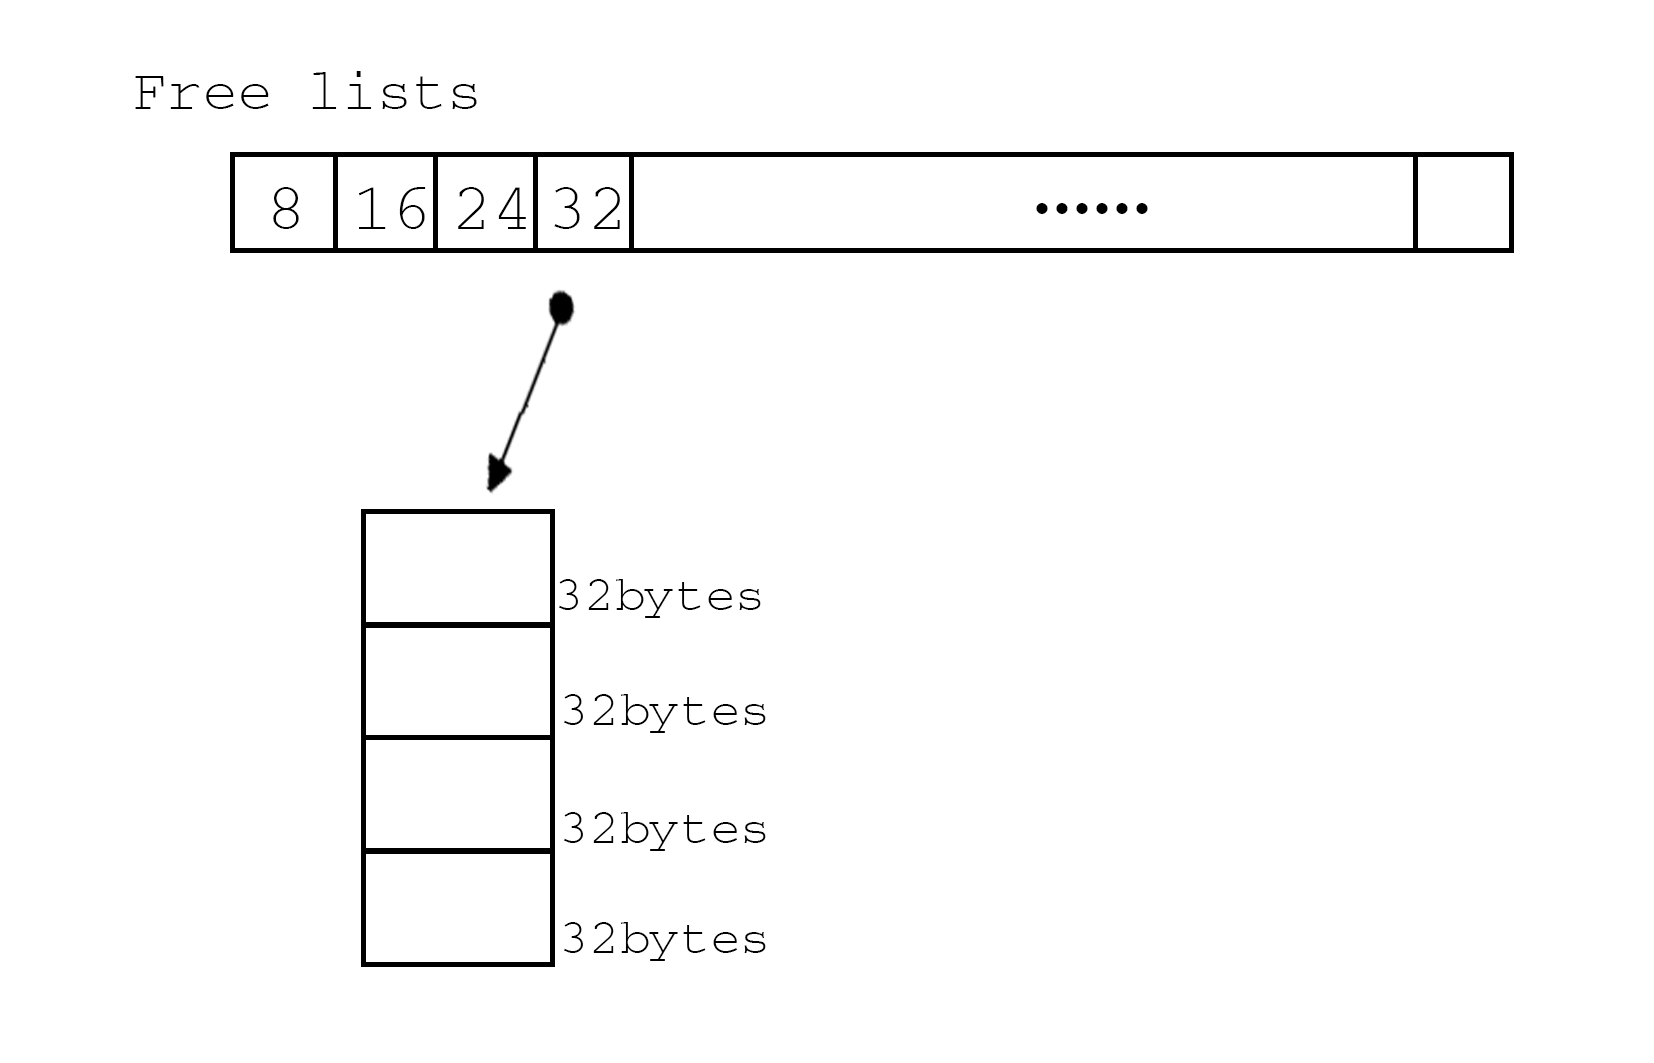
\includegraphics[width=10cm]{freelists.png}
		\caption{Free lists\label{freelist}}
		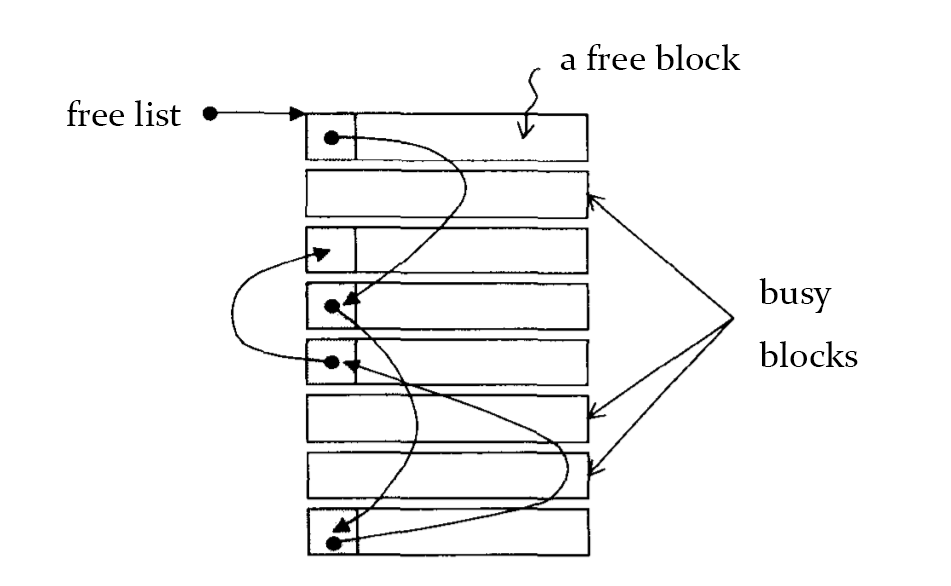
\includegraphics[width=10cm]{freelist.png}
		\caption{One linked list in free lists\label{linkedlist}}
	\end{figure}
\begin{lstlisting}
union Obj {
	Obj * freeListLink;
	char Data;
};
\end{lstlisting}
	
\end{itemize}

The allocation operation has two steps:
\begin{itemize}
	\item{\textbf{(1) Seek block in free list}}
	
	In this step, we simply round up size of required space, and search in freelists for free block. If it exits, return it directly. If not, call \texttt{refill} function to refill freelists, then return a free block after refillment.
\end{itemize}
\begin{center}
	\begin{algorithm}[H]
		\SetAlgoLined
		\label{LIS}
		\caption{Seek block in free list}
		input size N\\
		round up N to be multiple of 8\\
		Calculate corresponding index\\
		Get the pointer Ptr pointing to corresponding linked list\\
		\If{Ptr is not NULL}{Result $\leftarrow$ Ptr\\ Ptr $\leftarrow$ (Ptr$\rightarrow$next)}
		\Else{Result $\leftarrow$ refill freelists(N)}
		return Result
	\end{algorithm} 
\end{center}

\begin{itemize}
	\item{\textbf{(2) Refill free list with memory pool}}
	
	If a linked list is NULL for centain size block, we will refill it with many blocks. The number of blocks needed from memory pool depends.In general, an application usually calls a number of fixed size object,that means some freeList slot will be used more frequently. So, when refilling one freeList, we'd better give each size block differential treatment. The more one certain size used, the more blocks it will be refilled. To implement this idea, we use array \texttt{freeListCnt} to count the time of refillment for each size of block. And for next refillment, we will refill it with $$NumOfObj + Increment << Cnt$$ blocks (if memory pool allows). Then if a size usually run out of its blocks, it will get more blocks next time. It can reduce the times of function \texttt{refill} calling which is the costly operation.

	If space in memory pool is smaller than one block, we will use \texttt{::operator new} to allocate new memory pool. Similar with refillment, the size of new memory pool is effected by the size accumulated. More times we allocate a memory pool, bigger capacity we allocate.
	
\end{itemize}
\begin{center}
	\begin{algorithm}[H]
		\SetAlgoLined
		\caption{Refillment}
		bytesLeft $\leftarrow$ endFree - startFree\\
		NObj $\leftarrow$ NumOfObj + Increment << Cnt\\
		totalBytes $\leftarrow$ NObj * size of Type\\
		\If{bytesLeft > totalBytes}{Result $\leftarrow$ startFree\\startFree += totalBytes}
		\ElseIf{bytesLeft > size of block}{Result $\leftarrow$ startFree\\NObj $\leftarrow$ bytesLeft / size of block\\update totalbytes\\startFree += size of block}
		\Else{
			\If{bytesLeft > 0}{put left space into corresponding list}
			newBytes = roundUp(totalBytes * 2 + (heapSize >> 4))\\
			heapSize $\leftarrow$ heapSize + newBytes\\
			startFree $\leftarrow$ new (newBytes)\\
			update totalBytes and NObj\\
			endFree $\leftarrow$ startFree + newBytes\\
			Result $\leftarrow$ startFree
		}
		startFree += size of block\\
		\ForEach{i < NObj}{split a block from space\\
			add it to corresponding list\\
		i++}
		return Result
	\end{algorithm} 
\end{center}
\subsubsection{Third-level allocation}
In third-level allocation, there is also a freelists called \texttt{BFreelist}, some related defination is like this:
\begin{lstlisting}
enum{BigFreeLists = (SecondMaxBytes - MaxBytes)/Align};
static Obj * BFreeList[BigFreeLists];
\end{lstlisting}

When the required space size is between \texttt{SecondMaxBytes} and \texttt{MaxBytes}, second-level allocation works. Here, the \texttt{SecondMaxBytes} is 40960, and the \texttt{MaxBytes} is 4096. Everything else in third-level allocation is the same as that in second-level allocation, except \texttt{refill} operation:

Since when \texttt{BFreelist} runs out, those space size is too big to refill lists with sevel new blocks, and taking the less frequencies of allocation into consideration, we will just allocate one corresponding space block rather than \texttt{NumOfObj + Increment << Cnt}.

\vspace{1cm}

In class memoryPool, as we all see, those member variables and functions are all static. So we can use them directly without creating an instance. It guarantees that for one program, during the whole running process, only one memory pool is held, no matter how many objects are created, resized, or deleted. 

And all memory once has been allocated, it won't be returned until the program exits. In other word, the capacity of space that memory pool holds is always increasing.

What's more, the performance of our memory pool is depended on test program. If our allocator is tested with different test program, parameters (\texttt{Align, MaxBytes, SecondMaxBytes, NFreeLists, BigFreeLists, NumOfObj, Increment}) need ajusting to give a best performance. However, since memory pool is most used to optimize performance of one centain application, some prerequisite adjustment is common.

\section{Testing results}
We use vector and list which are most useful STL Containers to test our Memory Pool Allocator. We generate 12000 vector and 12000 list at random size. Then we stochastically choose 4000 container to be resized to a random size for both vector and list. We do same opertion to default allocator and calculate the optimizing rate $(T_d - T_m)/T_d$.
\begin{enumerate}
	\item First, we test these two allocator's performance. Obviously, allocator with memory pool is much better than default allocator as \ref{TestResult1} shows.
	\begin{figure}
		\centering
		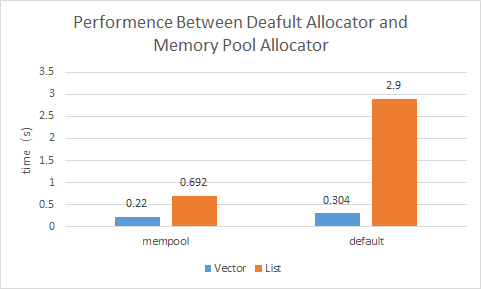
\includegraphics[]{performance.png}
		\caption{Two allocator's performance\label{TestResult1}}
	\end{figure}
	\item
	Second, we compare the performance between using normal distribution data and linear distribution data. For normal distribution data, we set mean = 256, variance = 10. Both up bound size is 500. We find that optimizing rate of vector is higher in normal distribution data obviously as \ref{TestResult2} shows. 
	\begin{figure}
		\centering
		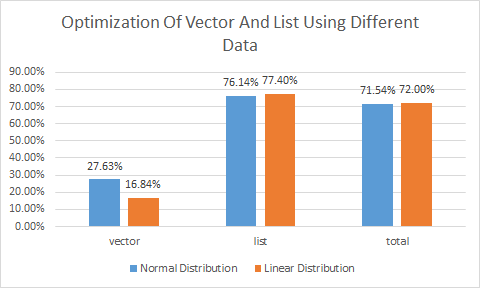
\includegraphics[]{figure1.png}
		\caption{Two data sets: normal distribution data and linear distribution data\label{TestResult2}}
	\end{figure}
	\item
	Then, We compare the performance between using Cnt and not.The conception of cnt has been introduced above.
	We find that using Cnt can do better in vector as \ref{TestResult3} shows.
	\begin{figure}
		\centering
		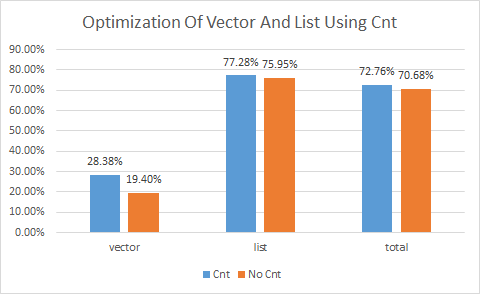
\includegraphics[]{figure2.png}
		\caption{Use Cnt and not\label{TestResult3}}
	\end{figure}
	\item
	Last, we compare the performance in different up bound of size. We find that with the up bound go up, optimizing rate goes up and to be convergent as \ref{TestResult4} shows.
	\begin{figure}
		\centering
		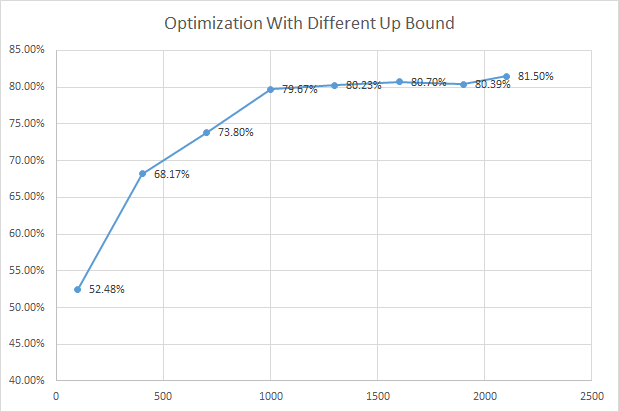
\includegraphics[]{figure3.png}
		\caption{Performance with different data size\label{TestResult4}}
	\end{figure}
\end{enumerate}

\section{Reference}

[1] WIKI Allocator(C++) https://en.wikipedia.org/wiki/Allocator\_(C++)

[2] 侯捷. SGI STL源码剖析. 华中科技大学出版社,2002


\end{document}